\section{Grundlagen}

\subsection{Marktrecherche}
Der größere Konkurrent bietet für seine Kunden, die ganze Messnetzwerke betreuen, bereits eine Lösung an.
Der sogenannte \enquote{Vaisala Observation Network Manager}\cite{observation-network-manager} bietet einen ähnlichen inhaltlichen Umfang.
Die Implementierung basiert ebenfalls auf Webtechnologien und bestätigt somit in diesem Punkt, den Ansatz seitens GRAW.

\subsection{Methodik und Vorgehensmodelle}
In kurzer Projektzeit von wenigen Monaten wurde ein umfangreicher und lauffähiger Prototyp bzw.\ ein MVP (Minimum Viable Product) erstellt.
Dabei wurde auf das Entwicklungsmodell XP (Extreme Programming) gesetzt, um auf den Aufwand für eine umfangreiche Planung zu verzichten.
Dafür wurden im Projektverlauf die bei XP üblichen fünf Werte und die 14 Prinzipien (Vergleiche~\cite{agile-prozesse}) berücksichtigt und auf das vorliegende Projekt angewandt.

Im Anschluss an die Implementierung der Software wurde, zusätzlich zu den daraus gewonnen praktischen Erfahrungswerten, eine Nutzwertanalyse durchgeführt, die sich methodisch an einem Praxisleitfaden~\cite{scoring-und-nutzwertanalysen} orientiert.
Ziel dieses Methodeneinsatzes ist es, das abschließende Fazit rationaler zu gestalten.
Zur Analyse zählt ein kurzer Vergleich von Nova mit anderen populären Laravel Admin-Panels (Vergleiche~\cite{the-guide-to-laravel-admin-panels}), die Auswahl und Gewichtung von Entscheidungskriterien, sowie das daraus resultierende Scoring.

\subsection{Technische Entwurfsmuster}

\subsubsection{MVC (Model View Controller)}
MVC ist ein etabliertes Entwurfsmuster für Benutzerinterfaces.
Durch eine klare Trennung der Zuständigkeiten werden Wartungen einfacher und können besser auf unterschiedliche Entwickler aufgeteilt werden.
Das Model ist nur zuständig für Daten und Business Logic, die View hingegen, nur für die Darstellung der Inhalte (\ref{fig:mvc})).
Der Controller ist das Bindeglied und routet Daten und Befehle zwischen den anderen beiden Bereichen.
(Vergleiche~\cite{mdn-glossary-mvc})

\begin{figure}[h!]
    \centering
    \caption{Model View Controller}
    \label{fig:mvc}
    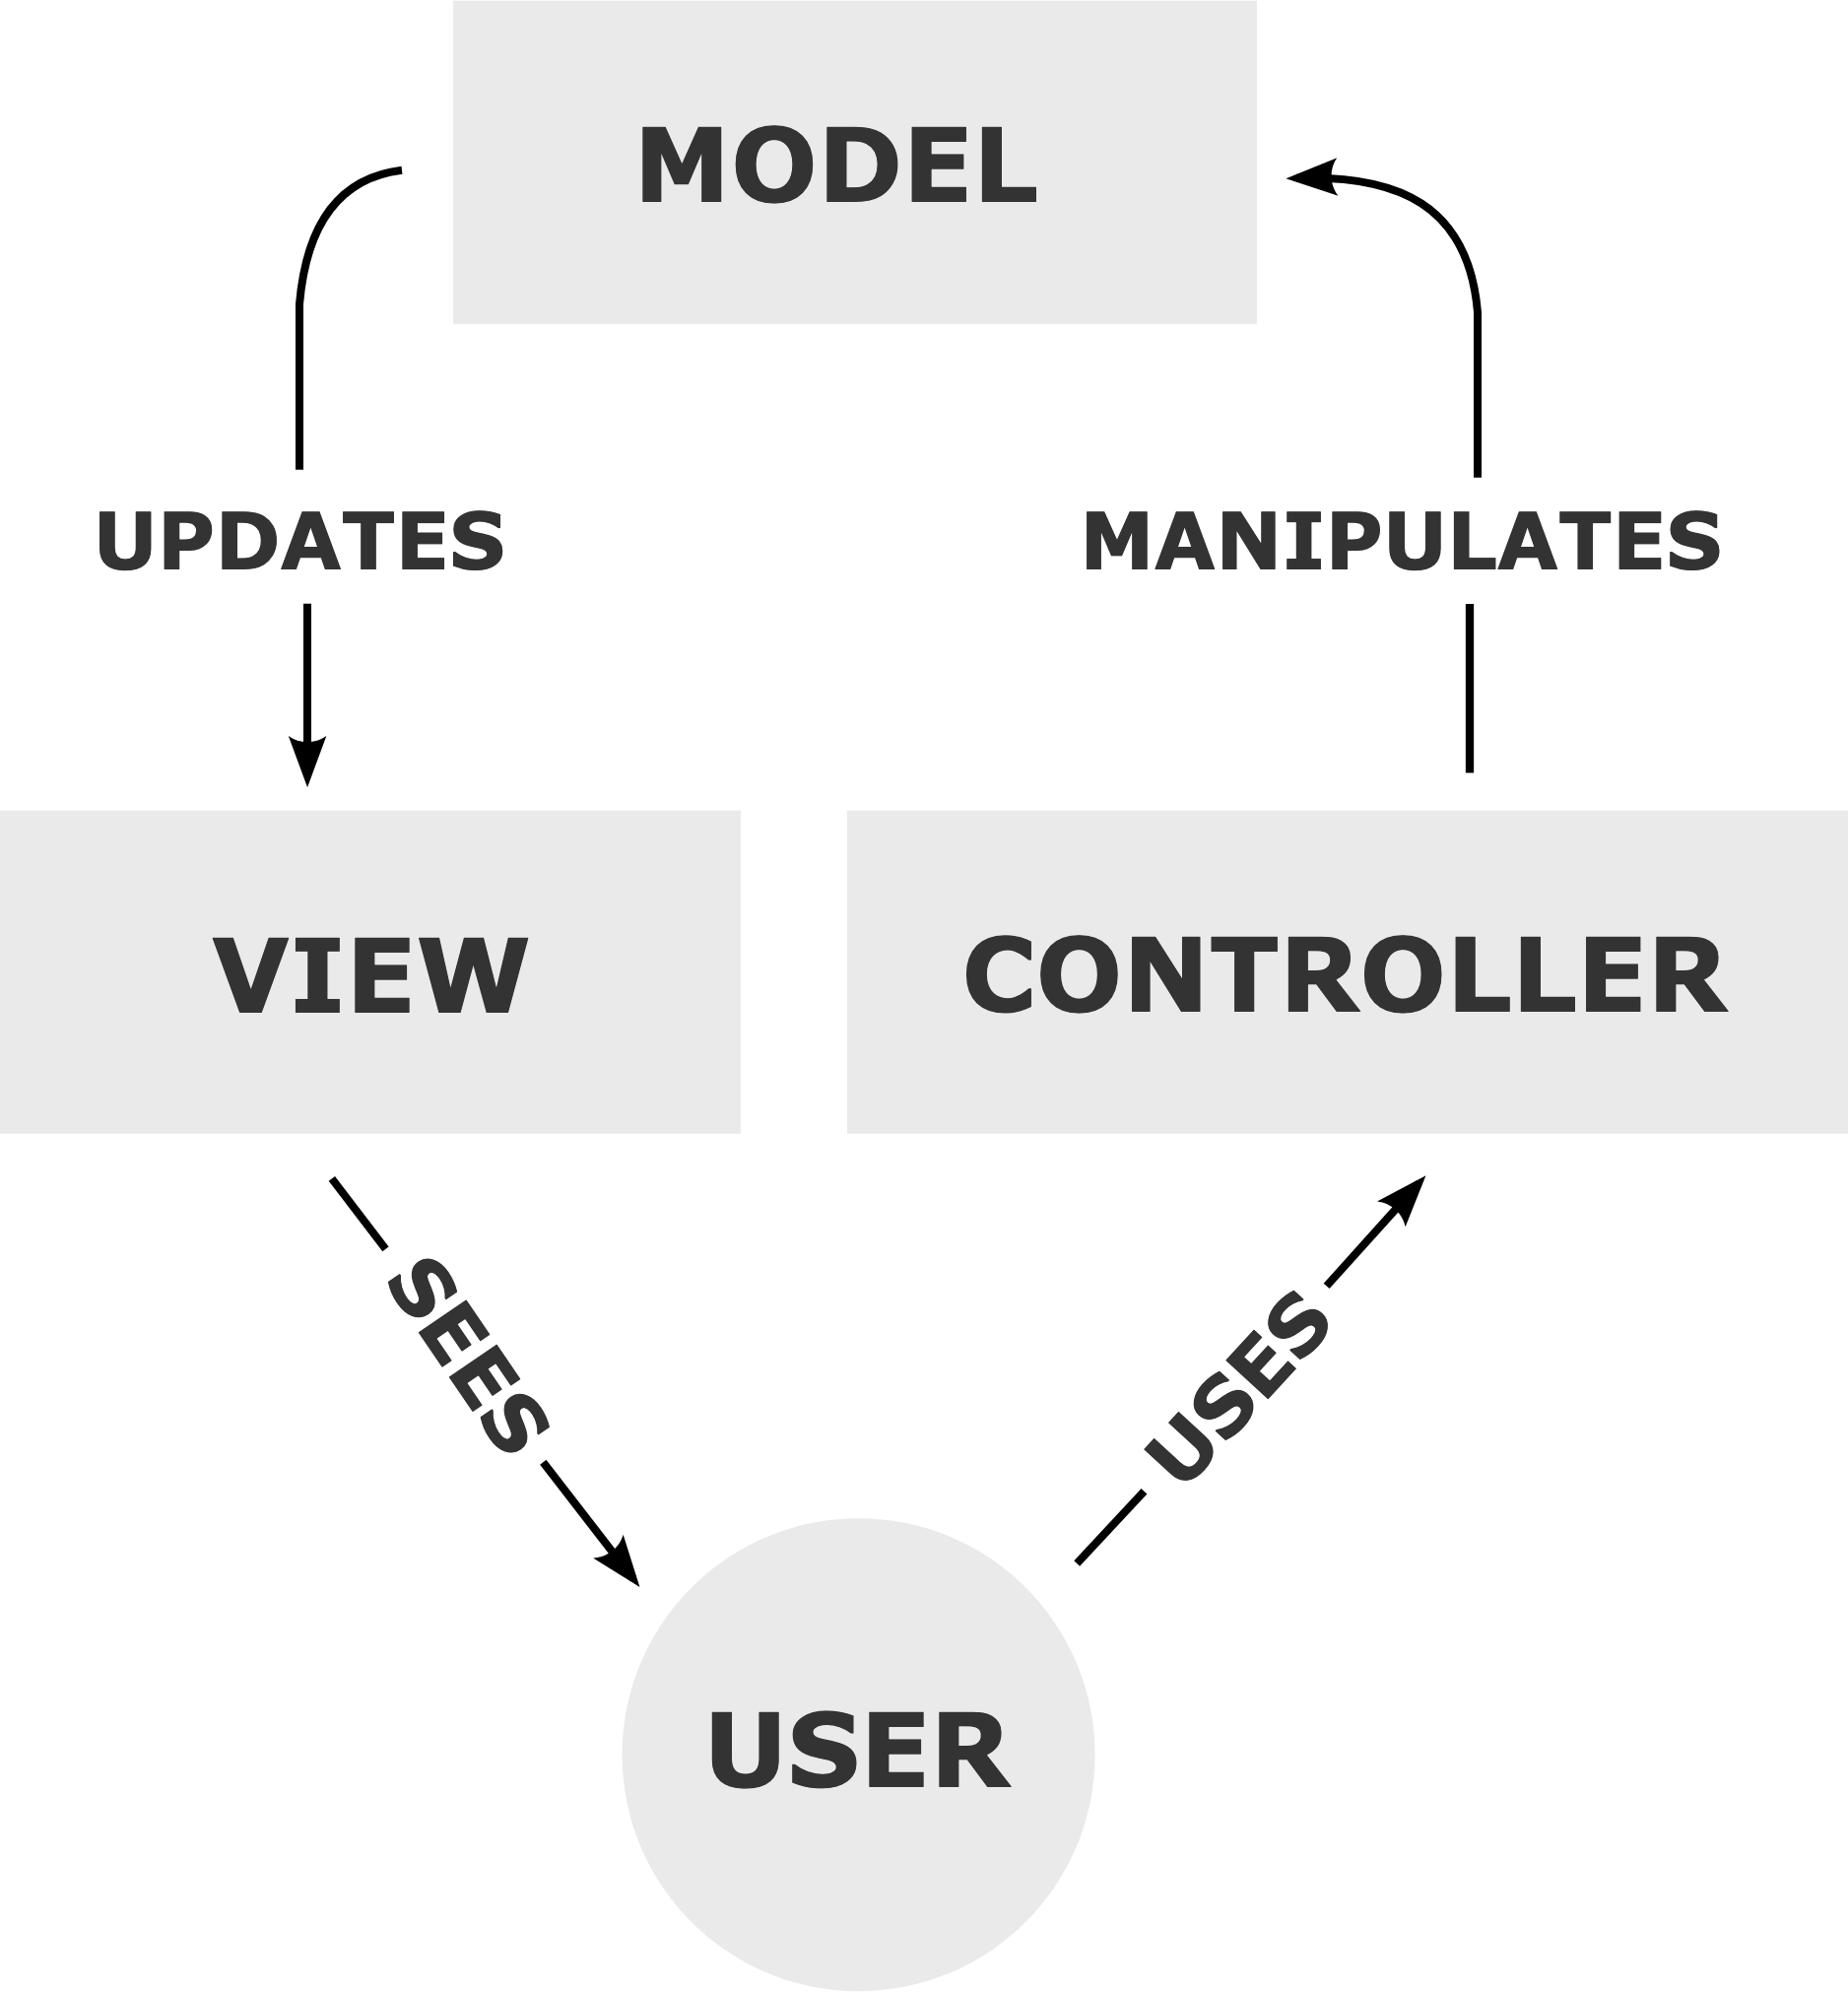
\includegraphics[scale=0.15]{assets/wikipedia_mvc_process}
\end{figure}

\newpage

\subsection{Technische Frameworks}

\subsubsection{Laravel}
Laravel ist ein kostenloses und quelloffenes Framework, für die Erstellung moderner PHP Anwendungen.
Es bietet ein starkes Toolset und eine umfangreiche Dokumentation sowie ein großes Ecosystem mit weiteren Funktionsbibliotheken und passenden Services.
Laravel verfügt u.a.\ über eine MVC Architektur, eingebaute Security Features, eine Templating Engine und eine ORM (Object Relational Mapping) Library.
In den letzten Jahren gewann es schnell an Popularität.
(Vergleiche~\cite{what-is-laravel})

\subsubsection{Nova}
Um Entwickler dabei zu unterstützen, besonders effizient und einfach, Administrationsinterfaces für Laravel Anwendungen zu entwickeln, wurde mit Nova ein kostenpflichtiges first-party Framework entwickelt und veröffentlicht (Vergleiche ~\cite{laravel-nova}).
Oftmals haben Laravel Anwendungen eine öffentliche Website, eine API (Programmierschnittstelle) und einen Administrationsbereich für die Verwaltung der Daten (Vergleiche~\cite{laravel-up-and-running}).
Mit Laravel lässt sich sehr gut eine API abdecken, ebenso ist es für öffentliche Websites designt.
Nova setzt also genau in dem Bereich an, den Entwickler in der Regel individuell aufbauen.

Für datengetriebene Verwaltungsanwendungen üblich und so auch grundsätzlich durch Laravel vorbereitet, ist eine MVC Architektur.
Mit Nova bleibt allerdings lediglich die Definition des Models, inklusive der Datenbankmigrationen.
Die übliche Programmlogik für Controller und View fällt weg.
Stattdessen werden Ressourcen mit Feldern definiert, die je einem Model zugeordnet werden.
Verglichen mit einer individuellen Implementierung lässt sich dadurch mit deutlich weniger Code die Verwaltung unterschiedlicher Ressourcen aufbauen.
